\subsection{HDFS [VI]}

The Hadoop Distributed File System (HDFS) \cite{HDFSArchitecture1} \cite{HDFSArchitecture2} is a distributed data storage that provides high throughput data access, fault-tolerance, ability to hold huge datasets consisting of large files.
The Apache Software Foundation has developed HDFS originally for its web search engine system - the Apache Nutch.
Today it is a widely-used distributed file system, that is an infrastructure for such distributed computational frameworks as Hadoop, Storm, etc.
HDFS allows to use cheap commodity hardware, because it does not require much computational or storage power for one particular node.
It is written in Java, hence, any platform with JVM \cite{JVM} can run HDFS's software.
HDFS supports standard hierarchical file organisation with directories and files.

\subsubsection{Use cases and requirements}

HDFS is designed for usage in the BigData world.
Applications, that use it, require high throughput data access.
They need to write and read files of gigabytes and terabytes in size fast.
HDFS is suitable for batch processing, and that is why low-latency is not a goal property.

Disk failures, and machine failures in general, happen more often, than we could think.
This is actually a normal case when we consider cluster of hundreds and even thousends of nodes.
The probability of a failure is complex and difficult to compute, but it is high enough, so that there are always machines in the large cluster, that are out of service.
This can happen also for the small number of nodes.
Because of that, the fault-tolerance, detecting of failed machines and recovering from unconsistent state of the file system is an inherent part of HDFS.

HDFS allows applications, that work with it, to operate with the large number of large files.
Files can be of gigabytes and terabytes in size, and there can be millions of files.
HDFS architecture lets to have high overall bandwidth working with such files.

HDFS has a simple file storage model.
It holds every file in a coherent way, so that it can be only written, and not changed any more.
Only one client writes the file to the file system, but many clients can then read it.
This model has a name \textit{write-once-read-many}, and it helps to provide high throughput data access.

HDFS lets an opportunity to move computations into the cluster, instead of moving data from the cluster to where computations are executing.
This is proven to be much more efficient, because moving data creates high network congestion.
When the data is of a very high volume it is important aspect to consider.

HDFS is written in Java, what allows to run it on practically all platforms and any hardware.
The only requirement for a machine to use it in the HDFS-cluster is that it has running JVM.

\subsubsection{General structure}

HDFS consists of two main elements: NameNode and DataNode.
These are applications that run on JVM.
They both do not require any particular operational system or hardware, and use local file system for storage of HDFS data pieces.

NameNode is a master programm of the cluster.
It stores meta information about the file system's namespace, regulates access of the clients to files, maintains consistent state of the file system, initializes operations like create, rename or delete file.
NameNode is of the highest importance, because its failure can be dangerous for the whole system.
It runs usually on a special separated machine.
The fact that there is only one master node greatly simplifies system's structure, its maintenance and analysis of errors.
Data never flows through the NameNode.

DataNode is a program that holds data.
Each machine in the cluster runs usually one DataNode.
DataNode executes read and write requests directly from the clients.
It also performs creation, deletion and replication of blocks, when NameNode gives such instructions.

DataNodes hold files in blocks.
Standard size of a block is 64 Mb.
Normally, each block resides on the different DataNode to provide high reading throughput.
Every file has replication factor, that defines the number of its replicas.
If replication factor is for example 3, than each block of this file has 3 copies on different machines.
This provides fault-tolerance in case of disk or other hardware failures.

Applications access HDFS using Client program, that provides interface to do write and read requests.
When Client writes, it asks NameNode to give a list of DataNodes to write replicas of the first block.
Then it accesses DataNode directly and makes write of the block.
DataNode in its turn sends write request of this block to another DataNode, that is in the list for replications.
And so on, until the block has all its replicas written.
When block is written, Client asks about new list of replicas for the next block.
When Client reads, it asks NameNode for the list of replicas of the first block, sorts it by the distance in the network topology, and then gets it from the nearest replica.
Then the same for the next block and so on.
You can see the overall structure of HDFS and the way of its functioning on the Figure~\ref{fig:HDFS}.

\begin{figure}[H]
  \centering
  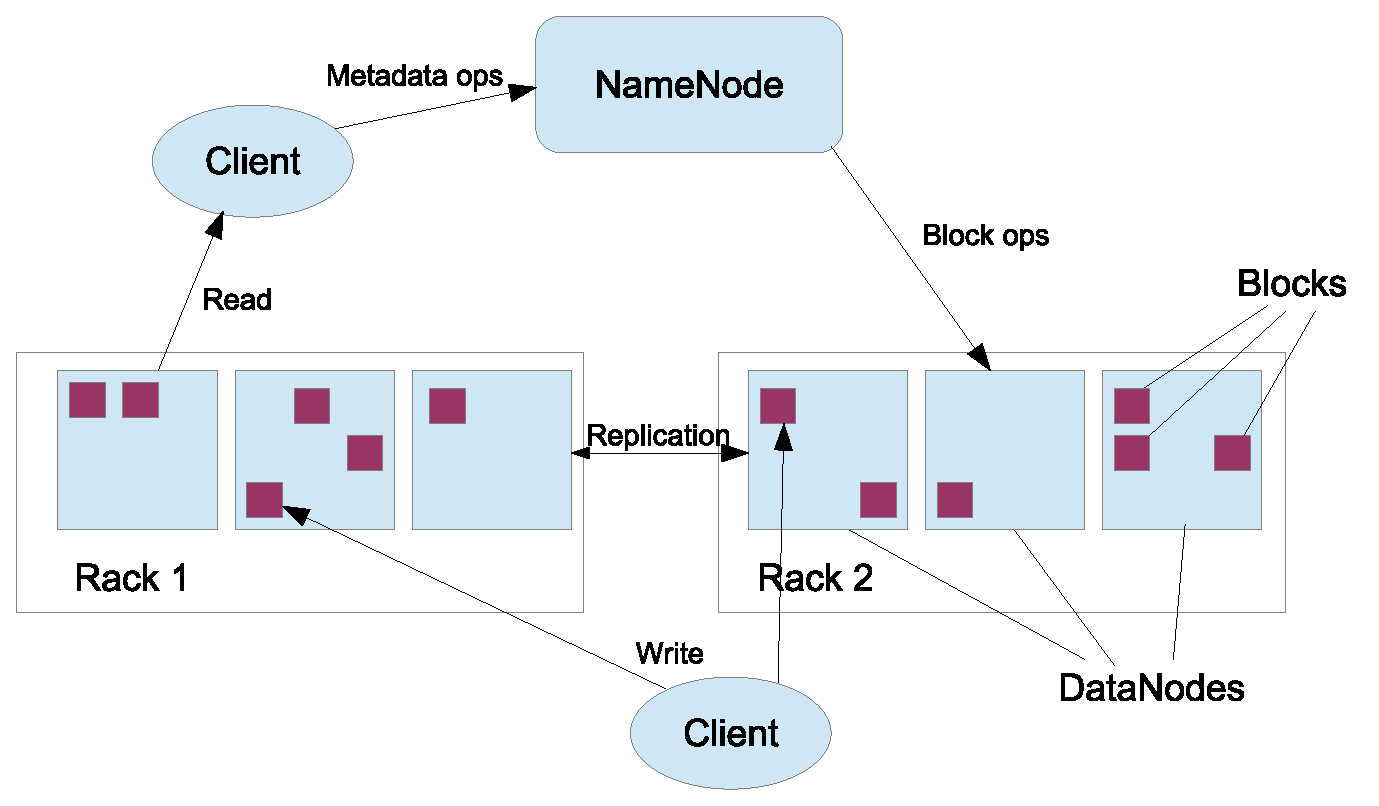
\includegraphics [width=0.8\textwidth]{images/HDFS}
  \caption{Overall structure of HDFS.}
  \label{fig:HDFS}
\end{figure}

\subsubsection{Replications}

HDFS stores large files reliably, so that failures of particular machines can lead to an unrecoverable lost of a part of a file with a very small probability.
It also provides high throughput, placing blocks of files onto different DataNodes, to give parallel access of many clients to many files in the cluster.
The number of replicas and the block size are configurable parameters for every file.
Replication factor also can be changed for already existing files.

Cluster consists of the number of racks.
Rack is a group of nodes, that reside usually near to each other physically.

The current replicas placement policy for the most common replication factor of 3 is as follows.
Put the first replica onto the DataNode in the rack, local for accessing client.
Put the second replica in the same rack, but onto the other DataNode.
Put the third replica onto the DataNode in another rack.
This approach gives both high fault-tolerance and near to optimal access rate.

\subsubsection{Robustness}

One of the main goals of HDFS is to provide fault-tolerance from hardware failures.
For this sake, each DataNode sends periodically a Heartbeat signal to the NameNode, to notify about its state.
If the DataNode's machine fails, the NameNode does not receive Heartbeat signal, and marks this DataNode as out of service.
The NameNode starts then re-replication of blocks, that resided on the failed machine.
Another condition to make re-replication is increase by the client of the replication factor of a particular file.

When the piece of data arrives to the client, it can be corrupted during transfer in the network or because of a IO failures.
To provide integrity of data, HDFS has a checksum mechanism.
When a block of file is written, its checksum is also written to the file system.
Then, when client reads a block, it also receives checksum and able to match file.

HDFS manages balance in the cluster.
If there are DataNodes that has free space below set threshold, file system moves part of data from that nodes to others, that have more free space.
This is done automatically, and does not allow to accumulate data in the part of the file system, decreasing its access throughput.

There is a staging mechanism in HDFS, that helps to avoid network congestion.
Client, that writes data to the file system, does it in portions.
It accumulates the whole block in the local cash file, and only then makes flush to the DataNode.